%% ========================================================================
%% Chapter 10: Memory Management & System Calls
%% ========================================================================
\chapter{Memory Management \& System Calls}
\label{ch:memory-and-syscalls}

Imagine your desk. Documents you are actively working on sit on the desk surface
--- this is analogous to \textbf{RAM}. When the desk gets full, some documents
are moved to a drawer to make room --- this is analogous to \textbf{swap}. If
all documents end up in the drawer and you keep going back and forth to retrieve
them, work slows to a crawl. That is a simple picture of how Linux manages memory.
In this chapter we will also learn about \textbf{system calls} --- the mechanism
programs use to request services from the kernel, and put the Bash skills from
Chapter~7 to work building real monitoring scripts.

\textbf{What You'll Learn}

By the end of this chapter, you will be able to:

\begin{enumerate}
    \item understand the virtual memory architecture of a Linux process;
    \item observe and interpret paging activity with \texttt{vmstat};
    \item create and configure swap space and the swappiness parameter;
    \item identify the processes with the highest memory usage;
    \item write a Bash script for automated memory monitoring;
    \item observe and analyse system calls using \texttt{strace}.
\end{enumerate}

\begin{notebox}
All lab tasks are run as a regular user unless the command explicitly uses
\texttt{sudo}. Create the working directory first:
\begin{lstlisting}
mkdir -p ~/lab-os/chapter08-memory
\end{lstlisting}
\end{notebox}

\section{Memory Architecture on Linux}

Every program running on Linux gets its own \textit{virtual address space}.
This means each program behaves as if it has private memory that cannot be
touched by other programs --- the kernel maps those virtual addresses to physical
RAM. The virtual address space is divided into several areas as shown in
\cref{fig:memory-layout}: the \textbf{Text Segment} holds code instructions
(read-only), the \textbf{Data Segment} holds global variables, the \textbf{Heap}
grows upward for dynamic allocation (\texttt{malloc()}), the \textbf{Stack}
grows downward for local variables and return addresses, and \textbf{Kernel Space}
is accessible only by the kernel.

\begin{figure}[H]
\centering
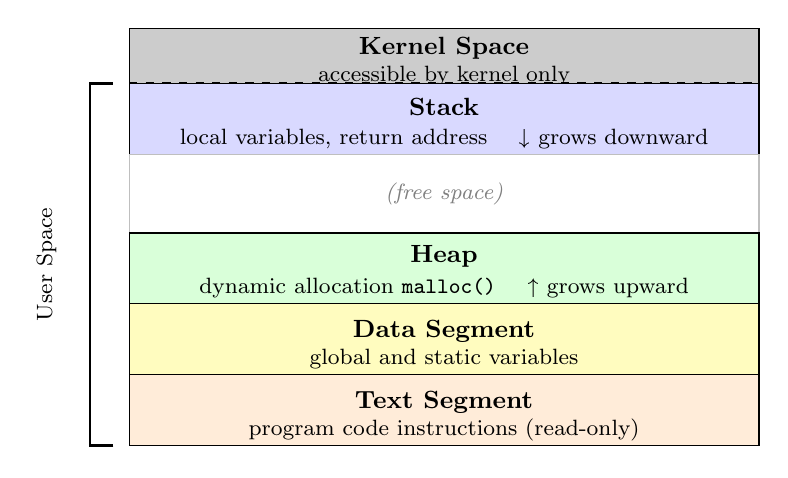
\begin{tikzpicture}[font=\small]
    \filldraw[fill=gray!40, draw=black] (0,5.0) rectangle (8,5.7);
    \node[font=\small\bfseries] at (4, 5.45) {Kernel Space};
    \node[font=\footnotesize] at (4, 5.1) {accessible by kernel only};
    \draw[dashed, thick] (0,5.0) -- (8,5.0);
    \filldraw[fill=blue!15, draw=black] (0,4.1) rectangle (8,5.0);
    \node[font=\small\bfseries] at (4, 4.7) {Stack};
    \node[font=\footnotesize] at (4, 4.3) {local variables, return address \quad ↓ grows downward};
    \draw[draw=gray!50] (0,3.1) rectangle (8,4.1);
    \node[font=\footnotesize\itshape, gray] at (4, 3.6) {(free space)};
    \filldraw[fill=green!15, draw=black] (0,2.2) rectangle (8,3.1);
    \node[font=\small\bfseries] at (4, 2.8) {Heap};
    \node[font=\footnotesize] at (4, 2.4) {dynamic allocation \texttt{malloc()} \quad ↑ grows upward};
    \filldraw[fill=yellow!25, draw=black] (0,1.3) rectangle (8,2.2);
    \node[font=\small\bfseries] at (4, 1.85) {Data Segment};
    \node[font=\footnotesize] at (4, 1.5) {global and static variables};
    \filldraw[fill=orange!15, draw=black] (0,0.4) rectangle (8,1.3);
    \node[font=\small\bfseries] at (4, 0.95) {Text Segment};
    \node[font=\footnotesize] at (4, 0.6) {program code instructions (read-only)};
    \draw[thick] (-0.2,0.4) -- (-0.5,0.4) -- (-0.5,5.0) -- (-0.2,5.0);
    \node[font=\footnotesize, rotate=90, anchor=south] at (-0.8, 2.7) {User Space};
\end{tikzpicture}
\caption{Virtual memory map of a Linux process. Each process has its own isolated
virtual address space, separate from all other processes.}
\label{fig:memory-layout}
\end{figure}

\begin{notebox}
Process isolation guarantees system stability. If one program crashes, the damage
is contained to that process --- other processes continue running normally.
\end{notebox}

\subsection*{Lab 8.1 Viewing Memory Usage}

Run \texttt{free -h} to see a summary of RAM and swap, then view kernel memory
details:

\begin{lstlisting}[caption={Memory summary and details}]
free -h
cat /proc/meminfo | head -n 20
\end{lstlisting}

The \texttt{free -h} output shows a \texttt{Mem} row (RAM) and a \texttt{Swap}
row. Key columns: \texttt{total} (total RAM), \texttt{used} (in use), \texttt{free}
(completely unused), \texttt{available} (truly available for new applications ---
use this, not \texttt{free}), and \texttt{buff/cache} (file cache reclaimed
automatically when needed).

\textit{Observe:} Calculate \texttt{available / total × 100\%}. Below 10\% means
the system is running low on memory. If the \texttt{used} column on the \texttt{Swap}
row is greater than 0, the kernel has already moved data to disk.

\begin{tipbox}
Do not worry if \texttt{used} appears large. Linux intentionally uses idle RAM as
a file cache to speed up disk access. Focus on \texttt{available}.
\end{tipbox}

\begin{challengebox}
An application server feels slow when many users are active. Use \texttt{free -h}
and \texttt{top} to investigate memory conditions. Inside \texttt{top}, press
\keystroke{M} to sort by memory. Record: the \texttt{available} value, whether
\texttt{Swap used} is greater than 0, and the name of the process with the highest
\texttt{\%MEM}. Write a brief analysis: is the server likely running out of memory?
\end{challengebox}

\section{Virtual Memory Management}

Imagine a large library. You can only place a few books on the reading table (RAM),
while the rest stay on the shelves (disk/swap). When you need a book from the shelf,
you fetch it and return another. That is how \textit{virtual memory} and
\textit{paging} work.

Data is divided into fixed-size blocks called \textbf{pages}. The kernel
automatically moves inactive pages to swap (\textit{swap out}) and loads them back
when needed (\textit{swap in}), as shown in \cref{fig:virtual-memory}. The command
\texttt{vmstat 1 5} reports virtual memory statistics every 1 second for 5 samples
--- the \texttt{si} (swap in) and \texttt{so} (swap out) columns are the primary
indicators of paging activity.

\begin{figure}[H]
\centering
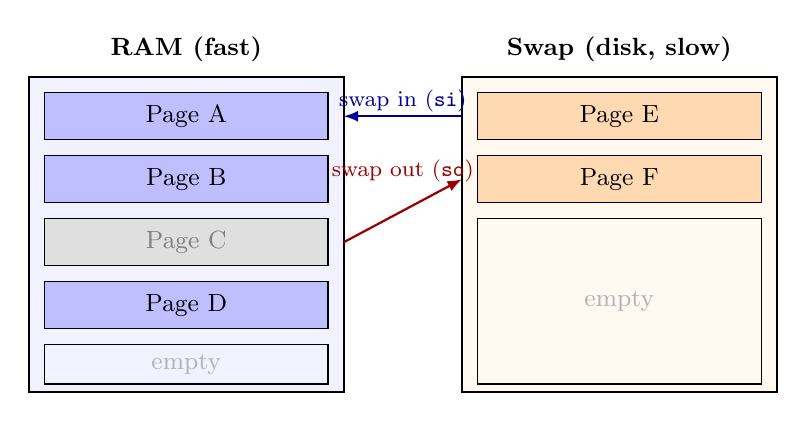
\begin{tikzpicture}[font=\small, >=latex]
    \draw[fill=blue!5, thick] (0,0) rectangle (4,4);
    \node[font=\small\bfseries] at (2, 4.35) {RAM (fast)};
    \filldraw[fill=blue!25]  (0.2,3.2) rectangle (3.8,3.8); \node at (2,3.5) {Page A};
    \filldraw[fill=blue!25]  (0.2,2.4) rectangle (3.8,3.0); \node at (2,2.7) {Page B};
    \filldraw[fill=gray!25]  (0.2,1.6) rectangle (3.8,2.2); \node[gray] at (2,1.9) {Page C};
    \filldraw[fill=blue!25]  (0.2,0.8) rectangle (3.8,1.4); \node at (2,1.1) {Page D};
    \draw (0.2,0.1) rectangle (3.8,0.6); \node[gray!60] at (2,0.35) {empty};
    \draw[fill=orange!5, thick] (5.5,0) rectangle (9.5,4);
    \node[font=\small\bfseries] at (7.5, 4.35) {Swap (disk, slow)};
    \filldraw[fill=orange!30] (5.7,3.2) rectangle (9.3,3.8); \node at (7.5,3.5) {Page E};
    \filldraw[fill=orange!30] (5.7,2.4) rectangle (9.3,3.0); \node at (7.5,2.7) {Page F};
    \draw (5.7,0.1) rectangle (9.3,2.2); \node[gray!60] at (7.5,1.15) {empty};
    \draw[->, thick, red!60!black] (4,1.9) -- (5.5,2.7);
    \node[font=\footnotesize, red!60!black] at (4.75, 2.8) {swap out (\texttt{so})};
    \draw[->, thick, blue!60!black] (5.5,3.5) -- (4,3.5);
    \node[font=\footnotesize, blue!60!black] at (4.75, 3.7) {swap in (\texttt{si})};
\end{tikzpicture}
\caption{Paging mechanism: the kernel moves inactive pages to swap when RAM is full,
and loads them back (\texttt{si}/\texttt{so} in \texttt{vmstat}) when needed.}
\label{fig:virtual-memory}
\end{figure}

\subsection*{Lab 8.2 Observing Paging Activity}

\begin{lstlisting}[caption={Virtual memory statistics}]
vmstat 1 5
\end{lstlisting}

Locate the \texttt{swap} section: sub-column \texttt{si} (KB/second from disk to
RAM) and \texttt{so} (KB/second from RAM to disk).

\textit{Observe:} On a system with adequate RAM, \texttt{si} and \texttt{so} are
always 0. If both are consistently greater than 0, the system is under serious
\textit{memory pressure} --- disk access is far slower than RAM so performance
drops sharply.

\begin{warningbox}
Persistently high \texttt{si} and \texttt{so} values indicate the system needs
more RAM. Solutions: add RAM, reduce concurrent processes, or optimise applications.
\end{warningbox}

\begin{challengebox}
Use the loop technique from Chapter~7 to record \texttt{si} and \texttt{so} values
every 5 seconds for 30 seconds, saving to \texttt{paging-log.txt}:
\begin{lstlisting}
for i in $(seq 1 6); do
    vmstat 1 2 | tail -1 >> paging-log.txt
    sleep 5
done
cat paging-log.txt
\end{lstlisting}
Did \texttt{si}/\texttt{so} change during monitoring? What does this tell you
about the system's memory condition?
\end{challengebox}

\section{Swap Space Configuration}

Swap space is an area on disk that acts as an extension of RAM. Swap prevents
the system from crashing when RAM is exhausted, but because it resides on disk,
access is far slower. Swap is a \textit{safety net}, not a replacement for RAM.

The \texttt{swappiness} parameter (0--100) controls how aggressively the kernel
uses swap. A high value (60--100, Linux default = 60) means the kernel quickly
moves data to swap even when RAM is still available. A low value (10--20) means
the kernel prefers RAM and only uses swap when truly necessary --- recommended for
application servers.

\subsection*{Lab 8.3 Creating and Configuring a Swap File}

\textbf{Step 1}: Create a 512~MB file, secure its permissions, format it as swap,
then activate it.

\begin{lstlisting}[caption={Creating and activating swap}]
sudo fallocate -l 512M /swapfile-chapter08
sudo chmod 600 /swapfile-chapter08
sudo mkswap /swapfile-chapter08
sudo swapon /swapfile-chapter08
\end{lstlisting}

\begin{warningbox}
\texttt{chmod 600} is \textbf{mandatory} before \texttt{mkswap}. A swap file can
contain fragments of sensitive data from program memory. Open permissions
(\texttt{644}) would allow other users to read the contents of that memory.
\end{warningbox}

\textbf{Step 2}: Verify the swap is active, then check and change swappiness.

\begin{lstlisting}[caption={Verify and set swappiness}]
swapon --show
free -h
cat /proc/sys/vm/swappiness
sudo sysctl vm.swappiness=10
cat /proc/sys/vm/swappiness
\end{lstlisting}

\textit{Observe:} The \texttt{/swapfile-chapter08} entry should appear in
\texttt{swapon --show} and the \texttt{total} on the \texttt{Swap} row in
\texttt{free -h} should increase by 512~MB. Confirm the swappiness value changed
from 60 to 10 in the second \texttt{cat} output.

\begin{notebox}
\texttt{sysctl} changes are temporary and lost after reboot. For a permanent
setting, add \texttt{vm.swappiness=10} to \texttt{/etc/sysctl.conf}.

Clean up after the lab:
\begin{lstlisting}
sudo swapoff /swapfile-chapter08
sudo rm /swapfile-chapter08
\end{lstlisting}
\end{notebox}

\begin{challengebox}
Create a second swap file of 128~MB, activate it, then try three different
swappiness values (1, 60, 100) --- note what changes in \texttt{swapon --show}
and \texttt{free -h} each time. Explain: when is swappiness 1 better than 100
for a web server? Clean up both swap files when done.
\end{challengebox}

\section{Memory Usage Monitoring}

Memory monitoring helps detect problems before they affect users. There are two
approaches: \textbf{real-time} with \texttt{top} (dynamic changes as they happen)
and \textbf{snapshot} with \texttt{ps aux} (process list at a single point in time,
suitable for reports). Key columns in \texttt{ps aux}: \texttt{\%MEM} (percentage
of total RAM), \texttt{RSS} (physical RAM actually in use right now, in KB), and
\texttt{VSZ} (total virtual memory allocated, always larger than RSS).

\subsection*{Lab 8.4 Memory Monitoring with a Script}

\textbf{Step 1}: Take a snapshot of processes sorted by highest memory usage.

\begin{lstlisting}[caption={Processes with the highest memory usage}]
ps aux --sort=-%mem | head
\end{lstlisting}

\textit{Observe:} The process on the second line (after the header) is the largest
memory consumer at that moment. Convert \texttt{RSS} from KB to MB (divide by 1024)
to understand how much physical RAM it is actually using.

\textbf{Step 2}: Build an automated monitoring script applying Chapter~7 concepts
(variables, \texttt{if} conditionals, and \texttt{awk} parsing).

\begin{lstlisting}[caption={Navigate to directory and open nano}]
cd ~/lab-os/chapter08-memory
nano monitor-memory.sh
\end{lstlisting}

\begin{lstlisting}[caption={Contents of monitor-memory.sh}]
#!/bin/bash
set -euo pipefail

THRESHOLD=20

echo "=== Memory Monitor ==="
date
echo

free -h
echo

AVAIL=$(free | awk '/Mem/ {printf "%d", $7/$2*100}')
if [ "$AVAIL" -lt "$THRESHOLD" ]; then
    echo "WARNING: Available memory is only ${AVAIL}%!"
else
    echo "Status: Available memory ${AVAIL}% (normal)"
fi
echo

echo "--- Top 5 Memory Processes ---"
ps aux --sort=-%mem | head -n 6 | tail -n 5
\end{lstlisting}

\begin{notebox}
Save: \keystroke{Ctrl+O} $\to$ \keystroke{Enter} $\to$ exit: \keystroke{Ctrl+X}.
\end{notebox}

\begin{lstlisting}[caption={Run the monitor script}]
chmod +x monitor-memory.sh
bash monitor-memory.sh
\end{lstlisting}

\textit{Observe:} The \texttt{awk} command reads column 7 (available) divided by
column 2 (total) from the \texttt{Mem} row, multiplied by 100 to produce an integer
percentage. Change \texttt{THRESHOLD} to \texttt{90} and run again --- does the
output change? Why?

\begin{challengebox}
Extend \texttt{monitor-memory.sh} so that each run saves a log to a file named
\texttt{memory-YYYYMMDD-HHMMSS.txt} using \texttt{date} (a technique from Chapter~7)
while still displaying output on screen with \texttt{tee}:
\begin{lstlisting}
LOGFILE="memory-$(date +%Y%m%d-%H%M%S).txt"
# ... script body ... | tee "$LOGFILE"
\end{lstlisting}
Run it twice and verify that two separate log files are created.
\end{challengebox}

\section{System Calls and User-Kernel Interaction}

Imagine a restaurant. You (the program) cannot walk directly into the kitchen
(the kernel) to cook your own food --- you must order through a waiter (the
system call). The waiter relays your order to the kitchen, ensures it is valid,
and brings the result back to your table.

That is how a system call works: a mechanism for programs in \textit{user space}
to request services from the kernel. A program cannot directly access hardware,
the filesystem, or kernel resources --- all requests must go through system calls.
The complete flow is shown in \cref{fig:syscall-flow}.

\begin{figure}[H]
\centering
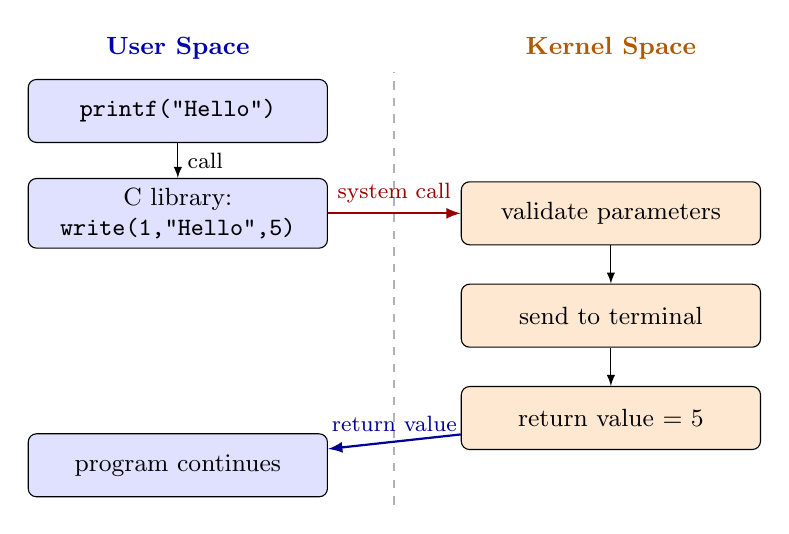
\begin{tikzpicture}[font=\small, >=latex,
    ub/.style={draw, fill=blue!12, rounded corners=3pt,
               minimum width=3.8cm, minimum height=0.8cm, align=center},
    kb/.style={draw, fill=orange!18, rounded corners=3pt,
               minimum width=3.8cm, minimum height=0.8cm, align=center}
]
    \node[font=\small\bfseries, blue!70!black]   at (2.0, 5.8) {User Space};
    \node[font=\small\bfseries, orange!70!black] at (7.5, 5.8) {Kernel Space};
    \draw[dashed, thick, gray!60] (4.75, 0.0) -- (4.75, 5.5);
    \node[ub] (app) at (2.0, 5.0) {\texttt{printf("Hello")}};
    \node[ub] (lib) at (2.0, 3.7) {C library:\\\texttt{write(1,"Hello",5)}};
    \node[ub] (fin) at (2.0, 0.5) {program continues};
    \node[kb] (val) at (7.5, 3.7) {validate parameters};
    \node[kb] (exe) at (7.5, 2.4) {send to terminal};
    \node[kb] (ret) at (7.5, 1.1) {return value = 5};
    \draw[->] (app) -- (lib) node[midway, right, font=\footnotesize] {call};
    \draw[->, thick, red!60!black] (lib) -- (val)
        node[midway, above, font=\footnotesize] {system call};
    \draw[->] (val) -- (exe);
    \draw[->] (exe) -- (ret);
    \draw[->, thick, blue!60!black] (ret) -- (fin)
        node[midway, above, font=\footnotesize] {return value};
\end{tikzpicture}
\caption{System call flow for \texttt{printf}: the user program requests a kernel
service through a controlled interface, not directly to hardware.}
\label{fig:syscall-flow}
\end{figure}

System calls are grouped by function: \textbf{Process Management}
(\texttt{fork}, \texttt{exec}, \texttt{exit}), \textbf{File Management}
(\texttt{open}, \texttt{read}, \texttt{write}, \texttt{close}),
\textbf{Memory Management} (\texttt{mmap}, \texttt{brk}), \textbf{Communication}
(\texttt{pipe}, \texttt{socket}), and \textbf{System Information}
(\texttt{getpid}, \texttt{uname}). The \texttt{strace} command lets us see every
system call a command makes, along with its arguments and return value.

\subsection*{Lab 8.5 Observing System Calls with strace}

\textbf{Step 1}: Simulate a file access failure due to permissions.

\begin{lstlisting}[caption={Simulate a permission error}]
mkdir -p ~/lab-os/chapter08-memory/syscall-case
cd ~/lab-os/chapter08-memory/syscall-case
echo "PORT=8080" > app.conf
chmod 000 app.conf
cat app.conf
\end{lstlisting}

The output \texttt{cat: app.conf: Permission denied} occurs because the system call
\texttt{openat()} failed --- the kernel rejected the request to open the file
because no read permission bit (\texttt{r}) is set. Restore permissions with
\texttt{chmod 644 app.conf}.

\textbf{Step 2}: Observe all system calls made by the \texttt{ls} command.

\begin{lstlisting}[caption={Detailed and summary system calls}]
strace ls 2>&1 | head -n 30
strace -c ls
\end{lstlisting}

Each line follows the format \texttt{syscallname(arguments) = return\_value}.
Example: \texttt{openat(AT\_FDCWD, "/etc/ld.so.cache", O\_RDONLY) = 3} means the
file was opened for reading successfully (file descriptor = 3). A value of
\texttt{-1 ENOENT} means the call failed because the file was not found.

\textit{Observe:} From the \texttt{strace -c} summary, which system call is invoked
most frequently? Are there any rows with \texttt{errors} greater than 0? Does the
program still run normally despite those failures?

\begin{tipbox}
Use \texttt{strace -c} for a quick overview. Use \texttt{strace} without \texttt{-c}
to see the exact order and arguments of every system call when diagnosing a specific
problem.
\end{tipbox}

\begin{challengebox}
Use \texttt{strace} with a filter to see only \texttt{openat} system calls:
\begin{lstlisting}
strace -e trace=openat cat /etc/hostname 2>&1
\end{lstlisting}
Count how many files are opened. Identify which succeed (positive return value)
and which fail (value \texttt{-1}). Why does \texttt{cat} open more than one file
just to display \texttt{/etc/hostname}?
\end{challengebox}

\section{Lab Assignment}

\textbf{General Instructions}: Complete all tasks in the following directory.

\begin{lstlisting}[caption={Preparing the assignment directory}]
mkdir -p ~/lab-os/chapter08-memory
cd ~/lab-os/chapter08-memory
\end{lstlisting}

\subsubsection{Assignment 8.1 System Memory Audit}

Create a script \texttt{memory-audit.sh} that automatically generates a memory
condition report.

\begin{lstlisting}[caption={Contents of memory-audit.sh}]
#!/bin/bash
set -euo pipefail

REPORT="memory-report.txt"

{
    echo "=== SYSTEM MEMORY REPORT ==="
    date
    echo
    echo "--- free -h Summary ---"
    free -h
    echo
    echo "--- /proc/meminfo ---"
    cat /proc/meminfo | head -n 20
} > "$REPORT"

echo "Report saved to: $REPORT"
cat "$REPORT"
\end{lstlisting}

\begin{lstlisting}[caption={Run the audit script}]
chmod +x memory-audit.sh
bash memory-audit.sh
\end{lstlisting}

Answer: (1) What is the \texttt{available / total} percentage? (2) Why is
\texttt{buff/cache} not counted as used memory from an application's perspective?
(3) What are the values of \texttt{SwapTotal} and \texttt{SwapFree} in
\texttt{/proc/meminfo}?

\subsubsection{Assignment 8.2 Identify Highest Memory Processes}

\begin{lstlisting}[caption={Save and display the top processes}]
ps aux --sort=-%mem | head -n 10 > top-memory-process.txt
cat top-memory-process.txt
\end{lstlisting}

Answer: (1) Which process is at the top? Record \texttt{\%MEM} and \texttt{RSS}.
(2) Convert \texttt{RSS} to MB. (3) Sum the \texttt{\%MEM} of the top 5 processes
--- what percentage of RAM do they consume together?

\subsubsection{Assignment 8.3 Create and Verify a Swap File}

\begin{lstlisting}[caption={Create and activate the assignment swap file}]
sudo fallocate -l 256M /swapfile-assign-chapter08
sudo chmod 600 /swapfile-assign-chapter08
sudo mkswap /swapfile-assign-chapter08
sudo swapon /swapfile-assign-chapter08
\end{lstlisting}

\begin{lstlisting}[caption={Verify and save the result}]
{
    echo "=== SWAP VERIFICATION ==="
    swapon --show
    echo
    free -h
} > swap-check.txt
cat swap-check.txt
\end{lstlisting}

\begin{notebox}
Clean up when done:\\
\texttt{sudo swapoff /swapfile-assign-chapter08 \&\& sudo rm /swapfile-assign-chapter08}
\end{notebox}

Answer: (1) Identify the \texttt{NAME}, \texttt{TYPE}, \texttt{SIZE}, and
\texttt{USED} columns. (2) Did \texttt{total} on the \texttt{Swap} row increase
by 256~MB? (3) Why is permission \texttt{600} important?

\subsubsection{Assignment 8.4 System Call Analysis with strace}

\begin{lstlisting}[caption={Save summary and detailed system calls}]
strace -c ls 2> strace-summary.txt
strace ls /etc 2> strace-ls-etc.txt
cat strace-summary.txt
\end{lstlisting}

Answer: (1) List at least 5 system calls with a brief description of each.
(2) Which system call is invoked most frequently? Why? (3) Are there any
\texttt{errors} greater than 0? Does the program still run normally?

\subsubsection{Assignment 8.5 Case Study: Diagnosing a Slow Server}

Create a diagnostic script that combines all checks from this chapter using
Bash functions from Chapter~7.

\begin{lstlisting}[caption={Open file with nano}]
nano ~/lab-os/chapter08-memory/diagnose-server.sh
\end{lstlisting}

\begin{longlisting}[language=bash, caption={Contents of diagnose-server.sh}]
#!/bin/bash
set -euo pipefail

REPORT="diagnose-server-slow.txt"
WARN_MEM=false
WARN_SWAP=0

check_memory() {
    echo "--- Memory Condition ---"
    free -h
    echo
    AVAIL_PCT=$(free | awk '/Mem/ {printf "%d", $7/$2*100}')
    if [ "$AVAIL_PCT" -lt 20 ]; then
        echo "WARNING: Available memory is only ${AVAIL_PCT}%"
        WARN_MEM=true
    fi
}

check_swap() {
    echo "--- Swap Usage ---"
    swapon --show 2>/dev/null || echo "No active swap"
    echo
    WARN_SWAP=$(free | awk '/Swap/ {print $3}')
    if [ "$WARN_SWAP" -gt 0 ]; then
        echo "INFO: Swap in use (${WARN_SWAP} kB)"
    fi
}

check_processes() {
    echo "--- Top 10 Memory Processes ---"
    ps aux --sort=-%mem | head -n 11
    echo
}

check_paging() {
    echo "--- Paging Activity (5 samples) ---"
    vmstat 1 5
    echo
}

summary() {
    echo "=== SUMMARY ==="
    if [ "$WARN_MEM" = true ]; then
        echo "- Memory: CRITICAL - immediate action required"
    else
        echo "- Memory: normal"
    fi
    if [ "$WARN_SWAP" -gt 0 ]; then
        echo "- Swap: in use - monitor paging activity"
    else
        echo "- Swap: not in use"
    fi
}

{
    echo "=== SERVER DIAGNOSTIC REPORT ==="
    date
    echo

    check_memory
    check_swap
    check_processes
    check_paging
    summary
} | tee "$REPORT"

echo
echo "Report saved to: $REPORT"
\end{longlisting}

\begin{notebox}
Save: \keystroke{Ctrl+O} $\to$ \keystroke{Enter} $\to$ exit: \keystroke{Ctrl+X}.
\end{notebox}

\begin{lstlisting}[caption={Run the diagnostic script}]
chmod +x ~/lab-os/chapter08-memory/diagnose-server.sh
bash diagnose-server.sh
\end{lstlisting}

Answer: (1) Explain the role of each function and why the diagnosis is split into
separate functions. (2) Based on the \texttt{SUMMARY} section, is the system normal
or critical? (3) Why does the script use \texttt{tee "\$REPORT"} instead of a plain
redirect \texttt{> "\$REPORT"}? (4) Is there any \texttt{si} or \texttt{so} activity
in \texttt{check\_paging}? What does it imply for server performance?

\section{References}

\begin{itemize}
    \item Nemeth et al., \textit{UNIX and Linux System Administration Handbook}.
    \item Linux Kernel documentation (\texttt{/proc}, \texttt{man 2 syscall}).
    \item Manual pages: \texttt{man free}, \texttt{man vmstat}, \texttt{man swapon},
    \texttt{man strace}, \texttt{man 2 syscall}.
\end{itemize}
